\documentclass[12pt,a4paper]{article}

% ============================================================
% Packages
% ============================================================
\usepackage[utf8]{inputenc}
\usepackage[T1]{fontenc}
\usepackage{lmodern}
\usepackage[english]{babel}
\usepackage{geometry}
\geometry{margin=2.5cm}
\usepackage{graphicx}
\usepackage{xcolor}
\usepackage{hyperref}
\usepackage{listings}
\usepackage{booktabs}
\usepackage{tabularx}
\usepackage{longtable}
\usepackage{enumitem}
\usepackage{tikz}
\usetikzlibrary{shapes.geometric, arrows.meta, positioning, fit, calc}
\usepackage{fancyhdr}
\usepackage{titlesec}
\usepackage{tocloft}
\usepackage{amsmath}
\usepackage{float}
\usepackage{caption}
\usepackage{subcaption}
\usepackage{pifont}
\usepackage{multicol}

% ============================================================
% Styling
% ============================================================
\definecolor{phantomblue}{RGB}{30, 58, 138}
\definecolor{phantomgray}{RGB}{100, 116, 139}
\definecolor{codebg}{RGB}{248, 250, 252}
\definecolor{codegreen}{RGB}{22, 163, 74}
\definecolor{codepurple}{RGB}{147, 51, 234}
\definecolor{criticalred}{RGB}{220, 38, 38}
\definecolor{highorg}{RGB}{234, 88, 12}
\definecolor{mediumyel}{RGB}{202, 138, 4}
\definecolor{lowblue}{RGB}{37, 99, 235}

\hypersetup{
    colorlinks=true,
    linkcolor=phantomblue,
    urlcolor=phantomblue,
    citecolor=phantomblue,
}

\lstset{
    basicstyle=\ttfamily\small,
    backgroundcolor=\color{codebg},
    frame=single,
    rulecolor=\color{phantomgray!40},
    keywordstyle=\color{codepurple}\bfseries,
    commentstyle=\color{codegreen},
    stringstyle=\color{criticalred},
    breaklines=true,
    showstringspaces=false,
    tabsize=4,
    numbers=left,
    numberstyle=\tiny\color{phantomgray},
}

\pagestyle{fancy}
\fancyhf{}
\fancyhead[L]{\small\textcolor{phantomgray}{Phantom -- Technical Report}}
\fancyhead[R]{\small\textcolor{phantomgray}{v0.9.15}}
\fancyfoot[C]{\thepage}
\renewcommand{\headrulewidth}{0.4pt}

\titleformat{\section}{\Large\bfseries\color{phantomblue}}{\thesection}{1em}{}
\titleformat{\subsection}{\large\bfseries\color{phantomblue!80}}{\thesubsection}{1em}{}
\titleformat{\subsubsection}{\normalsize\bfseries\color{phantomblue!60}}{\thesubsubsection}{1em}{}

% ============================================================
% Document
% ============================================================
\begin{document}

% ============================================================
% Title Page
% ============================================================
\begin{titlepage}
\centering
\vspace*{2cm}

{\Huge\bfseries\textcolor{phantomblue}{Phantom}\par}
\vspace{0.5cm}
{\LARGE Autonomous AI-Powered\\Penetration Testing System\par}
\vspace{1.5cm}

{\Large\textbf{Technical Report \& Security Audit}\par}
\vspace{0.5cm}
{\large Version 0.9.15 -- Security Hardened\par}
\vspace{2cm}

\begin{tabular}{rl}
\textbf{Author:} & Gadouri Roumaissa \\
\textbf{Email:} & r\_gadouri@estin.dz \\
\textbf{Institution:} & ESTIN -- \'Ecole Sup\'erieure en Sciences et \\
                       & Technologies de l'Informatique et du Num\'erique \\
\textbf{Date:} & \today \\
\textbf{License:} & Apache License 2.0 \\
\end{tabular}

\vfill
{\small
This document provides a comprehensive technical description of the Phantom
autonomous penetration testing system, including its architecture, execution
model, security audit findings, remediation measures, strengths, and
future research directions.
}
\end{titlepage}

% ============================================================
% Table of Contents
% ============================================================
\newpage
\tableofcontents
\newpage

% ============================================================
% 1. Executive Summary
% ============================================================
\section{Executive Summary}

Phantom is an autonomous AI-powered penetration testing system that combines
large language models (LLMs) with a multi-agent graph architecture to conduct
end-to-end security assessments of web applications, networks, and APIs without
continuous human intervention.

Unlike traditional automated scanners that follow rigid rule sets, Phantom
leverages LLM-based reasoning to dynamically plan attack strategies, chain
exploits, and adapt to unexpected application behaviors---mimicking the
workflow of an experienced human penetration tester.

\textbf{Key metrics:}
\begin{itemize}[nosep]
    \item \textbf{20+ integrated security tools} (nmap, nuclei, sqlmap, ffuf, katana, etc.)
    \item \textbf{Multi-agent graph} with dynamic subagent spawning
    \item \textbf{Docker-sandboxed} execution environment (Kali Linux)
    \item \textbf{Multi-provider LLM support} (OpenAI, Anthropic, Google, Ollama, etc.)
    \item \textbf{100+ vulnerability classes} supported via skill library
    \item \textbf{21 security findings} identified and remediated in v0.9.15
\end{itemize}

% ============================================================
% 2. System Overview
% ============================================================
\section{System Overview}

\subsection{What is Phantom?}

Phantom is a command-line tool and Docker-based system designed to:
\begin{enumerate}[nosep]
    \item Accept a target specification (URL, IP, domain)
    \item Autonomously conduct a full penetration test
    \item Generate a professional vulnerability report
\end{enumerate}

The system operates through an \textbf{agentic AI loop}: a root agent plans
high-level strategy, spawns specialized child agents for specific tasks
(reconnaissance, vulnerability scanning, exploitation, verification), and
aggregates results into a final report.

\subsection{Technology Stack}

\begin{table}[H]
\centering
\caption{Phantom Technology Stack}
\begin{tabularx}{\textwidth}{lX}
\toprule
\textbf{Component} & \textbf{Technology} \\
\midrule
Core Language & Python 3.12 \\
LLM Integration & LiteLLM (multi-provider abstraction) \\
Agent Framework & Custom multi-agent graph (LangGraph-inspired) \\
Sandbox & Docker (Kali Linux rolling container) \\
Proxy/Interceptor & Caido (HTTP interception proxy) \\
Web Automation & Playwright (headless browser) \\
API Server & FastAPI + Uvicorn \\
Configuration & Pydantic models + YAML \\
Package Manager & Poetry \\
\bottomrule
\end{tabularx}
\end{table}

\subsection{Supported LLM Providers}

Phantom supports any LLM accessible through LiteLLM:
\begin{multicols}{2}
\begin{itemize}[nosep]
    \item OpenAI (GPT-4o, o3-mini)
    \item Anthropic (Claude 4 Sonnet/Opus)
    \item Google (Gemini 2.5 Pro/Flash)
    \item Ollama (local models)
    \item DeepSeek
    \item Groq
    \item OpenRouter
    \item Any OpenAI-compatible API
\end{itemize}
\end{multicols}

% ============================================================
% 3. Architecture
% ============================================================
\section{Architecture}

\subsection{High-Level Architecture}

\begin{figure}[H]
\centering
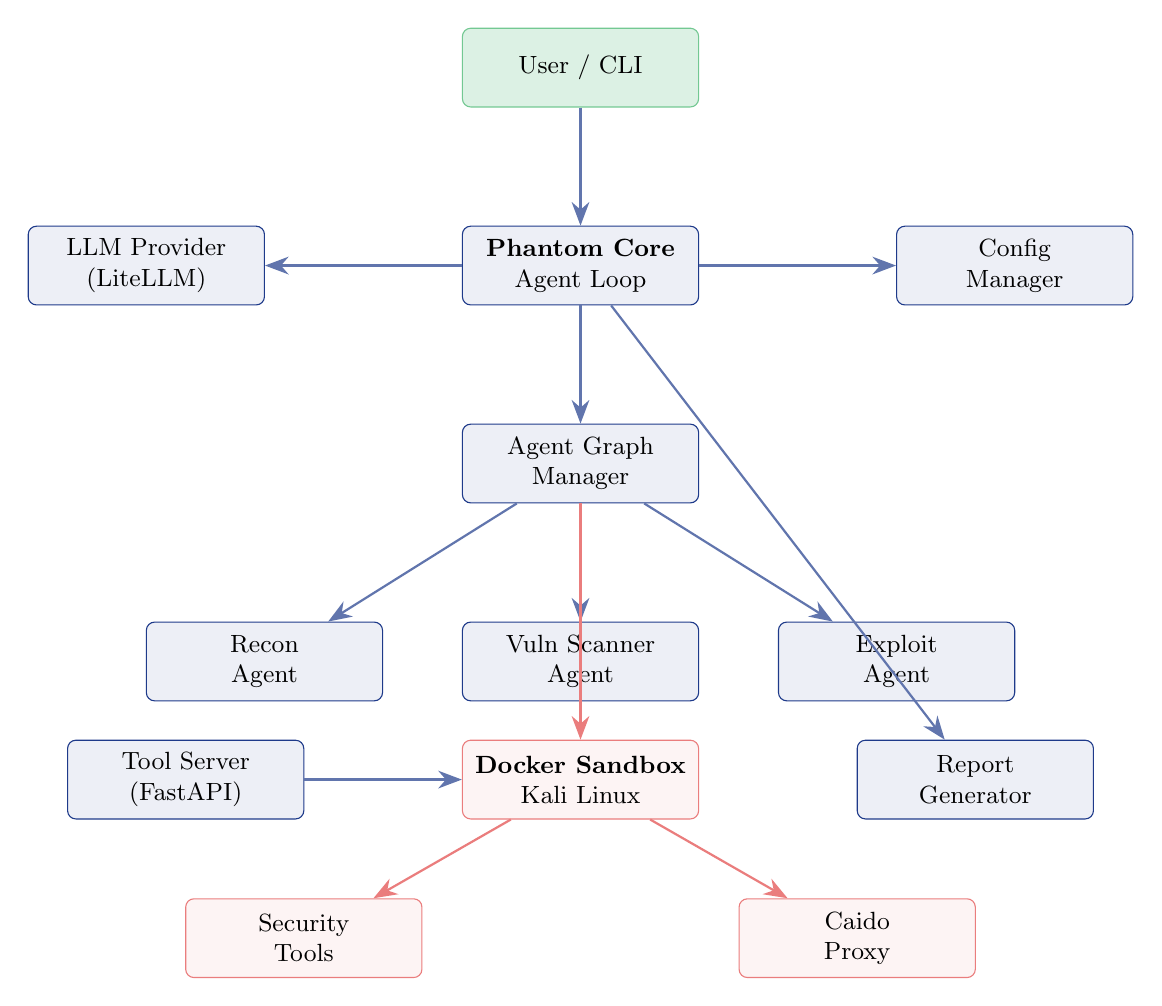
\begin{tikzpicture}[
    node distance=1.5cm and 2cm,
    box/.style={rectangle, draw=phantomblue, fill=phantomblue!8,
                minimum width=3cm, minimum height=1cm, align=center,
                rounded corners=3pt, font=\small},
    sandbox/.style={rectangle, draw=criticalred!60, fill=criticalred!5,
                    minimum width=3cm, minimum height=1cm, align=center,
                    rounded corners=3pt, font=\small},
    arr/.style={-{Stealth[length=3mm]}, thick, phantomblue!70},
    darr/.style={-{Stealth[length=3mm]}, thick, criticalred!60},
]

% User
\node[box, fill=codegreen!15, draw=codegreen!60] (user) {User / CLI};

% Core
\node[box, below=of user] (phantom) {\textbf{Phantom Core}\\Agent Loop};
\node[box, left=2.5cm of phantom] (llm) {LLM Provider\\(LiteLLM)};
\node[box, right=2.5cm of phantom] (config) {Config\\Manager};

% Agent Graph
\node[box, below=of phantom] (graph) {Agent Graph\\Manager};
\node[box, below left=1.5cm and 1cm of graph] (recon) {Recon\\Agent};
\node[box, below=of graph] (vuln) {Vuln Scanner\\Agent};
\node[box, below right=1.5cm and 1cm of graph] (exploit) {Exploit\\Agent};

% Sandbox
\node[sandbox, below=3cm of graph] (docker) {\textbf{Docker Sandbox}\\Kali Linux};
\node[sandbox, below left=1cm and 0.5cm of docker] (tools) {Security\\Tools};
\node[sandbox, below right=1cm and 0.5cm of docker] (proxy) {Caido\\Proxy};

% Tool Server
\node[box, left=2cm of docker] (toolsrv) {Tool Server\\(FastAPI)};

% Report
\node[box, right=2cm of docker] (report) {Report\\Generator};

% Arrows
\draw[arr] (user) -- (phantom);
\draw[arr] (phantom) -- (llm);
\draw[arr] (phantom) -- (config);
\draw[arr] (phantom) -- (graph);
\draw[arr] (graph) -- (recon);
\draw[arr] (graph) -- (vuln);
\draw[arr] (graph) -- (exploit);
\draw[darr] (graph) -- (docker);
\draw[darr] (docker) -- (tools);
\draw[darr] (docker) -- (proxy);
\draw[arr] (toolsrv) -- (docker);
\draw[arr] (phantom) -- (report);

\end{tikzpicture}
\caption{Phantom High-Level Architecture}
\label{fig:arch}
\end{figure}

\subsection{Multi-Agent Graph Architecture}

Phantom uses a \textbf{directed acyclic graph (DAG)} of AI agents, where:

\begin{itemize}[nosep]
    \item The \textbf{Root Agent} acts as the orchestrator, maintaining the
          overall scan strategy and spawning child agents
    \item \textbf{Child Agents} are specialized for specific tasks (recon,
          vulnerability scanning, exploitation, verification)
    \item Agents communicate through a \textbf{message-passing} system with
          sanitized inter-agent content (PHT-002 fix)
    \item Each agent has its own \textbf{conversation history} and \textbf{state}
\end{itemize}

\begin{figure}[H]
\centering
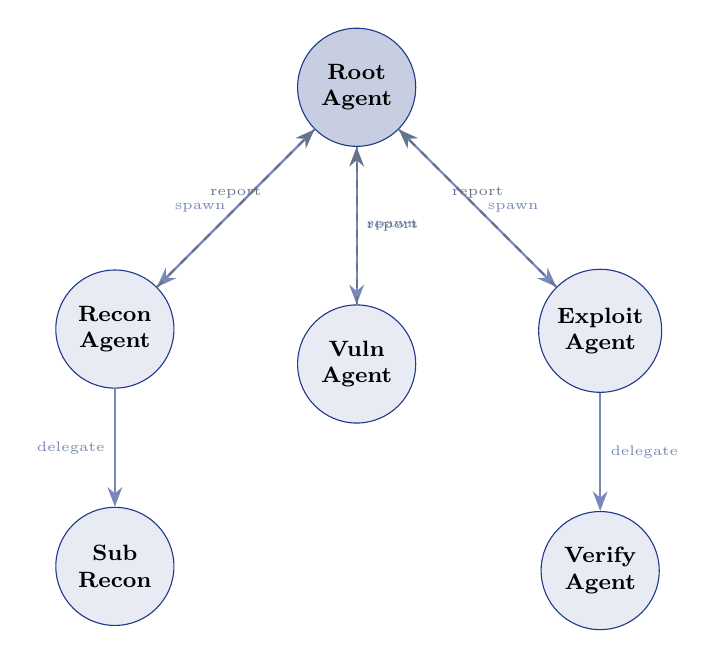
\begin{tikzpicture}[
    agent/.style={circle, draw=phantomblue, fill=phantomblue!10,
                  minimum size=1.5cm, font=\footnotesize\bfseries, align=center},
    arr/.style={-{Stealth[length=2.5mm]}, thick, phantomblue!60},
]

\node[agent, fill=phantomblue!25] (root) {Root\\Agent};
\node[agent, below left=2cm and 2cm of root] (a1) {Recon\\Agent};
\node[agent, below=2cm of root] (a2) {Vuln\\Agent};
\node[agent, below right=2cm and 2cm of root] (a3) {Exploit\\Agent};
\node[agent, below=1.5cm of a1] (a4) {Sub\\Recon};
\node[agent, below=1.5cm of a3] (a5) {Verify\\Agent};

\draw[arr] (root) -- node[left, font=\tiny] {spawn} (a1);
\draw[arr] (root) -- node[right, font=\tiny] {spawn} (a2);
\draw[arr] (root) -- node[right, font=\tiny] {spawn} (a3);
\draw[arr] (a1) -- node[left, font=\tiny] {delegate} (a4);
\draw[arr] (a3) -- node[right, font=\tiny] {delegate} (a5);
\draw[arr, dashed, phantomgray] (a1) -- node[above, font=\tiny] {report} (root);
\draw[arr, dashed, phantomgray] (a2) -- node[right, font=\tiny] {report} (root);
\draw[arr, dashed, phantomgray] (a3) -- node[above, font=\tiny] {report} (root);

\end{tikzpicture}
\caption{Multi-Agent Graph with Dynamic Subagent Spawning}
\label{fig:agent-graph}
\end{figure}

\subsection{Docker Sandbox Environment}

All security tools execute inside a \textbf{Docker container} based on Kali
Linux. This provides:

\begin{itemize}[nosep]
    \item \textbf{Isolation}: Tools cannot affect the host system
    \item \textbf{Reproducibility}: Consistent environment across deployments
    \item \textbf{Security}: Resource limits (4GB RAM, 2 CPUs, 512 PIDs) prevent abuse
    \item \textbf{Tool availability}: Pre-installed security tools (nmap, sqlmap, nuclei, etc.)
\end{itemize}

% ============================================================
% 4. Execution Flow
% ============================================================
\section{Execution Flow}

\subsection{Scan Lifecycle}

\begin{figure}[H]
\centering
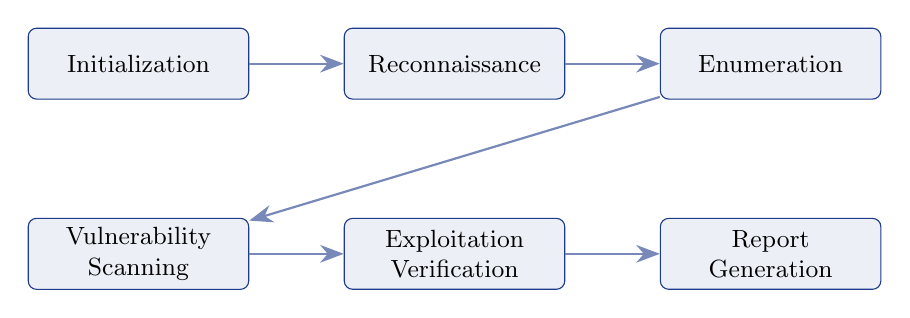
\begin{tikzpicture}[
    phase/.style={rectangle, draw=phantomblue, fill=phantomblue!8,
                  minimum width=2.8cm, minimum height=0.9cm, align=center,
                  rounded corners=3pt, font=\small},
    arr/.style={-{Stealth[length=3mm]}, thick, phantomblue!60},
]

\node[phase] (init) {Initialization};
\node[phase, right=1.2cm of init] (recon) {Reconnaissance};
\node[phase, right=1.2cm of recon] (enum) {Enumeration};
\node[phase, below=1.5cm of init] (vuln) {Vulnerability\\Scanning};
\node[phase, right=1.2cm of vuln] (exploit) {Exploitation\\Verification};
\node[phase, right=1.2cm of exploit] (report) {Report\\Generation};

\draw[arr] (init) -- (recon);
\draw[arr] (recon) -- (enum);
\draw[arr] (enum) -- (vuln);
\draw[arr] (vuln) -- (exploit);
\draw[arr] (exploit) -- (report);

\end{tikzpicture}
\caption{Phantom Scan Lifecycle Phases}
\label{fig:lifecycle}
\end{figure}

\subsection{Agent Iteration Loop}

Each agent follows a \textbf{think-act-observe} loop:

\begin{enumerate}
    \item \textbf{Think}: The LLM analyzes the current conversation history,
          available tools, and discovered information to decide the next action
    \item \textbf{Act}: The agent executes one or more tool invocations
          (e.g., run nmap, browse a webpage, test for SQL injection)
    \item \textbf{Observe}: Tool results are added to the conversation history,
          and the agent re-evaluates its strategy
    \item \textbf{Repeat}: Until the agent determines its task is complete
          or a cost/iteration limit is reached
\end{enumerate}

\subsection{Data Flow}

\begin{figure}[H]
\centering
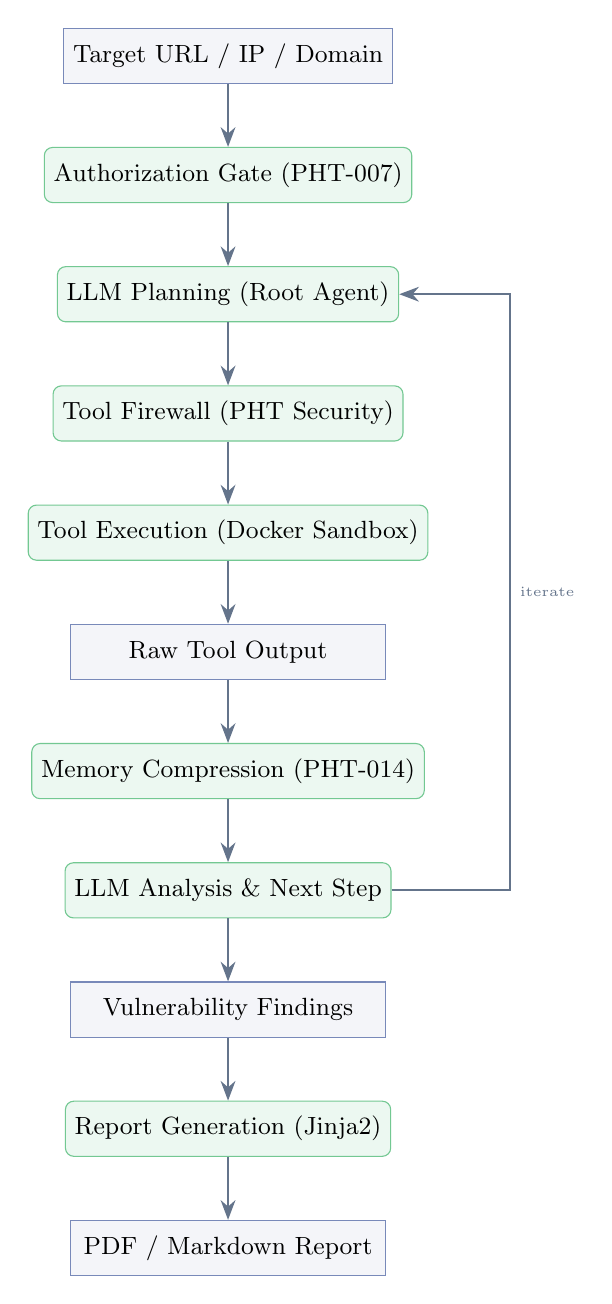
\begin{tikzpicture}[
    node distance=0.8cm,
    data/.style={rectangle, draw=phantomblue!60, fill=phantomblue!5,
                 minimum width=4cm, minimum height=0.7cm, align=center,
                 font=\small},
    process/.style={rectangle, draw=codegreen!60, fill=codegreen!8,
                    minimum width=4cm, minimum height=0.7cm, align=center,
                    rounded corners=3pt, font=\small},
    arr/.style={-{Stealth[length=2.5mm]}, thick, phantomgray},
]

\node[data] (input) {Target URL / IP / Domain};
\node[process, below=of input] (auth) {Authorization Gate (PHT-007)};
\node[process, below=of auth] (plan) {LLM Planning (Root Agent)};
\node[process, below=of plan] (fw) {Tool Firewall (PHT Security)};
\node[process, below=of fw] (exec) {Tool Execution (Docker Sandbox)};
\node[data, below=of exec] (results) {Raw Tool Output};
\node[process, below=of results] (compress) {Memory Compression (PHT-014)};
\node[process, below=of compress] (analyze) {LLM Analysis \& Next Step};
\node[data, below=of analyze] (findings) {Vulnerability Findings};
\node[process, below=of findings] (report) {Report Generation (Jinja2)};
\node[data, below=of report] (output) {PDF / Markdown Report};

\draw[arr] (input) -- (auth);
\draw[arr] (auth) -- (plan);
\draw[arr] (plan) -- (fw);
\draw[arr] (fw) -- (exec);
\draw[arr] (exec) -- (results);
\draw[arr] (results) -- (compress);
\draw[arr] (compress) -- (analyze);
\draw[arr] (analyze) -- (findings);
\draw[arr] (analyze.east) -- ++(1.5,0) |- node[right, font=\tiny, pos=0.25] {iterate} (plan.east);
\draw[arr] (findings) -- (report);
\draw[arr] (report) -- (output);

\end{tikzpicture}
\caption{End-to-End Data Flow}
\label{fig:dataflow}
\end{figure}

% ============================================================
% 5. Security Architecture
% ============================================================
\section{Security Architecture}

\subsection{Threat Model}

As an autonomous AI system executing offensive security tools, Phantom
faces unique security challenges:

\begin{enumerate}[nosep]
    \item \textbf{Prompt Injection}: Malicious web content could inject
          instructions into the LLM to alter scanning behavior
    \item \textbf{Inter-Agent Injection}: A compromised child agent could
          attempt to manipulate its parent
    \item \textbf{Command Injection}: User-controlled input flowing into
          shell commands without sanitization
    \item \textbf{Resource Exhaustion}: Infinite loops or excessive tool
          execution consuming unbounded resources
    \item \textbf{Data Exfiltration}: Sensitive scan data leaking through
          unencrypted storage or network exposure
\end{enumerate}

\subsection{Security Controls (v0.9.15)}

\begin{table}[H]
\centering
\caption{Security Controls Implemented}
\begin{tabularx}{\textwidth}{lX}
\toprule
\textbf{Control} & \textbf{Description} \\
\midrule
Authorization Gate & Interactive consent + auth file + legal disclaimer before scanning \\
Tool Invocation Firewall & Validates all tool arguments for injection patterns, length, scope \\
Cost Controller & Tracks token usage and cost; aborts at configurable limits \\
Loop Detector & Identifies repeated tool calls, cyclic patterns, stagnation \\
SSRF Protection & DNS pre-resolution to prevent rebinding attacks \\
Command Sanitization & \texttt{shlex.quote()} + regex validation on all shell parameters \\
Inter-Agent Sanitization & 5-layer content sanitization with prompt injection pattern detection \\
Rate Limiter & 60 req/60s per IP on tool server endpoint \\
HMAC Audit Chain & Tamper-evident audit log with HMAC-SHA256 chaining \\
Encryption at Rest & Optional Fernet (AES-128-CBC) for knowledge store data \\
Resource Limits & Docker: 4GB RAM, 2 CPUs, 512 PIDs, 20GB storage \\
\bottomrule
\end{tabularx}
\end{table}

\subsection{Defense in Depth}

\begin{figure}[H]
\centering
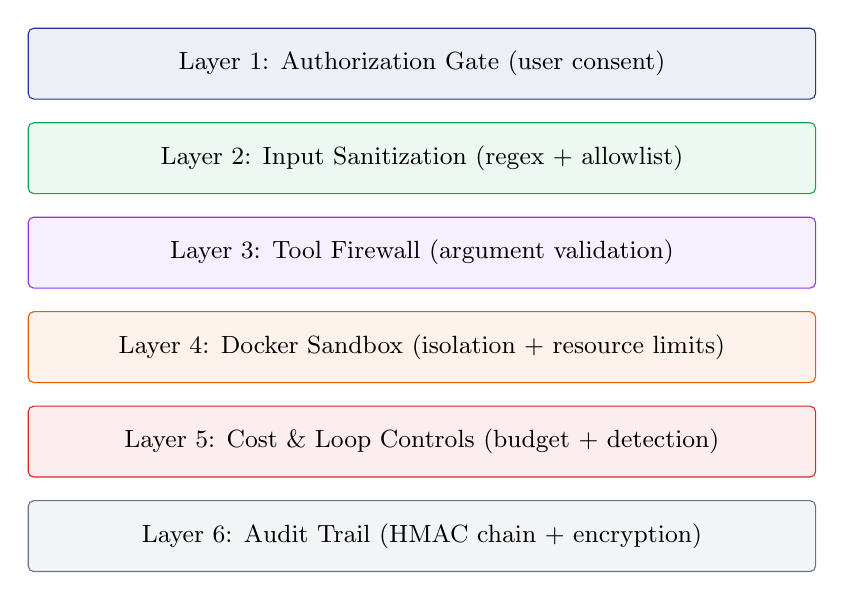
\begin{tikzpicture}[
    layer/.style={rectangle, draw=#1, fill=#1!8, minimum width=10cm,
                  minimum height=0.9cm, align=center, rounded corners=2pt,
                  font=\small},
]

\node[layer=phantomblue] (l1) at (0,0) {Layer 1: Authorization Gate (user consent)};
\node[layer=codegreen] (l2) at (0,-1.2) {Layer 2: Input Sanitization (regex + allowlist)};
\node[layer=codepurple] (l3) at (0,-2.4) {Layer 3: Tool Firewall (argument validation)};
\node[layer=highorg] (l4) at (0,-3.6) {Layer 4: Docker Sandbox (isolation + resource limits)};
\node[layer=criticalred] (l5) at (0,-4.8) {Layer 5: Cost \& Loop Controls (budget + detection)};
\node[layer=phantomgray] (l6) at (0,-6.0) {Layer 6: Audit Trail (HMAC chain + encryption)};

\end{tikzpicture}
\caption{Defense-in-Depth Security Layers}
\label{fig:defense}
\end{figure}

% ============================================================
% 6. Security Audit & Remediation
% ============================================================
\section{Security Audit \& Remediation}

A comprehensive security audit was conducted on Phantom v0.9.14, identifying
21 findings across critical, high, medium, and low severities. All findings
were verified against actual source code and remediated in v0.9.15.

\subsection{Findings Summary}

\begin{table}[H]
\centering
\caption{Security Audit Findings by Severity}
\begin{tabular}{lccc}
\toprule
\textbf{Severity} & \textbf{Found} & \textbf{Fixed} & \textbf{Status} \\
\midrule
\textcolor{criticalred}{\textbf{Critical}} & 2 & 2 & \ding{51} All Fixed \\
\textcolor{highorg}{\textbf{High}} & 5 & 5 & \ding{51} All Fixed \\
\textcolor{mediumyel}{\textbf{Medium}} & 9 & 9 & \ding{51} All Fixed \\
\textcolor{lowblue}{\textbf{Low}} & 3 & 3 & \ding{51} All Fixed \\
\textbf{Informational} & 2 & 2 & \ding{51} All Fixed \\
\midrule
\textbf{Total} & \textbf{21} & \textbf{21} & \textbf{100\% Remediated} \\
\bottomrule
\end{tabular}
\end{table}

\subsection{Critical Findings \& Fixes}

\subsubsection{PHT-001: Shell Command Injection via Nmap Parameters}

\begin{itemize}[nosep]
    \item \textbf{Severity}: Critical (CVSS 9.1)
    \item \textbf{Location}: \texttt{phantom/tools/security/nmap\_tool.py}
    \item \textbf{Issue}: Port and script parameters were passed directly to
          shell commands without validation, allowing injection via
          \texttt{80; rm -rf /}
    \item \textbf{Fix}: Added regex validators (\texttt{\_VALID\_PORTS\_RE},
          \texttt{\_VALID\_SCRIPTS\_RE}) and \texttt{shlex.quote()} for all
          user-controlled parameters
\end{itemize}

\subsubsection{PHT-002: Inter-Agent Prompt Injection}

\begin{itemize}[nosep]
    \item \textbf{Severity}: Critical (CVSS 8.6)
    \item \textbf{Location}: \texttt{phantom/agents/base\_agent.py}
    \item \textbf{Issue}: Messages between agents used XML wrapper that could
          be forged; only simple tag-stripping was applied
    \item \textbf{Fix}: Implemented 5-layer sanitization
          (\texttt{\_sanitize\_inter\_agent\_content}): XML tag stripping,
          markdown code block removal, tool-call syntax removal, 14 prompt
          injection pattern detection, 8000-character length cap
\end{itemize}

\subsection{High-Severity Findings \& Fixes}

\begin{longtable}{p{1.5cm}p{3.5cm}p{8cm}}
\toprule
\textbf{ID} & \textbf{Finding} & \textbf{Remediation} \\
\midrule
\endhead
PHT-003 & SSRF via DNS Rebinding & Added \texttt{socket.getaddrinfo()} DNS pre-resolution before IP comparison \\
PHT-004 & Auth Header Injection & Applied \texttt{shlex.quote()} to header values + dangerous char stripping \\
PHT-005 & Tool Server on 0.0.0.0 & Changed default bind to \texttt{127.0.0.1} in server and entrypoint \\
PHT-006 & No Resource Limits & Added Docker limits: 4GB RAM, 2 CPUs, 512 PIDs, 20GB storage \\
PHT-007 & No Authorization Gate & Created \texttt{AuthorizationGate} module with consent, auth file, legal disclaimer \\
\bottomrule
\end{longtable}

% ============================================================
% 7. Tool Integration
% ============================================================
\section{Tool Integration}

Phantom integrates 20+ security tools through a \textbf{unified tool registry}:

\begin{table}[H]
\centering
\caption{Integrated Security Tools}
\begin{tabularx}{\textwidth}{llX}
\toprule
\textbf{Category} & \textbf{Tool} & \textbf{Purpose} \\
\midrule
Reconnaissance & nmap & Port scanning, service detection \\
               & subfinder & Subdomain enumeration \\
               & httpx & HTTP probing and technology detection \\
               & katana & Web crawler \\
Vulnerability & nuclei & Template-based vulnerability scanning \\
              & sqlmap & SQL injection testing \\
              & dalfox & XSS vulnerability scanner \\
Web Testing & ffuf & Directory/parameter fuzzing \\
            & Playwright & Browser automation for dynamic content \\
            & Caido Proxy & HTTP traffic interception and replay \\
API Testing & arjun & API parameter discovery \\
            & Postman/curl & Direct API request testing \\
\bottomrule
\end{tabularx}
\end{table}

% ============================================================
% 8. Strengths
% ============================================================
\section{Strengths}

\begin{enumerate}
    \item \textbf{Autonomous Reasoning}: Unlike rule-based scanners, Phantom
          uses LLM reasoning to dynamically adapt its testing strategy based
          on observed responses, mimicking expert pentest decision-making
    
    \item \textbf{Multi-Agent Collaboration}: The graph-based agent system
          enables parallel work streams with specialized agents, scaling
          the assessment efficiently
    
    \item \textbf{Comprehensive Tool Integration}: 20+ tools covering the
          full penetration testing lifecycle from reconnaissance to
          exploitation to reporting
    
    \item \textbf{Provider Agnostic}: Supports any LLM through LiteLLM,
          from cloud APIs to local Ollama deployments, enabling use in
          air-gapped environments
    
    \item \textbf{Security-Hardened}: 6-layer defense-in-depth architecture
          with authorization gate, tool firewall, cost controls, loop
          detection, HMAC audit trail, and encryption at rest
    
    \item \textbf{Knowledge Persistence}: Cross-scan knowledge store enables
          learning from past assessments and avoiding redundant testing
    
    \item \textbf{Skill Library}: 100+ vulnerability-specific skill documents
          guide the LLM with expert methodology per vulnerability class
    
    \item \textbf{Professional Reporting}: Automated generation of
          structured vulnerability reports with CVSS scoring, evidence,
          and remediation guidance
\end{enumerate}

% ============================================================
% 9. Limitations
% ============================================================
\section{Current Limitations}

\begin{enumerate}
    \item \textbf{LLM Hallucination}: The AI may occasionally misinterpret
          tool output or generate false positive vulnerability claims
    \item \textbf{Cost}: Extended scans with frontier models (GPT-4o, Claude)
          can accumulate significant API costs (\$5--\$50 per comprehensive scan)
    \item \textbf{Scope Creep}: Without strict scope enforcement, the agent
          may wander to related but out-of-scope targets
    \item \textbf{Determinism}: Identical scans may produce different results
          due to LLM stochasticity
    \item \textbf{Complex Exploit Chains}: Multi-step exploitation requiring
          deep application logic understanding remains challenging
\end{enumerate}

% ============================================================
% 10. Future Work
% ============================================================
\section{Future Work}

\subsection{Short-Term (6 months)}
\begin{itemize}[nosep]
    \item \textbf{Formal Verification}: Mathematical proof of agent boundary
          invariants using model checking
    \item \textbf{MCP Integration}: Model Context Protocol for standardized
          tool communication
    \item \textbf{Benchmark Suite}: Reproducible evaluation against OWASP
          WebGoat, DVWA, and HackTheBox targets
    \item \textbf{Cost Optimization}: Implement speculative decoding and
          prompt caching to reduce LLM costs by 60\%
\end{itemize}

\subsection{Medium-Term (1 year)}
\begin{itemize}[nosep]
    \item \textbf{Collaborative Mode}: Human-in-the-loop option where the
          AI requests human guidance for ambiguous decisions
    \item \textbf{RAG-Enhanced Skills}: Retrieve-and-generate skill
          documents from a vector database of CVE/CWE knowledge
    \item \textbf{API Spec Ingestion}: Automatic OpenAPI/Swagger spec
          parsing for targeted API testing
    \item \textbf{Continuous Monitoring}: Periodic re-scanning with
          differential reporting
\end{itemize}

\subsection{Long-Term (2+ years)}
\begin{itemize}[nosep]
    \item \textbf{Exploit Synthesis}: AI-generated proof-of-concept exploits
          for discovered vulnerabilities
    \item \textbf{Multi-Target Campaigns}: Coordinated assessments across
          multiple related systems
    \item \textbf{Defensive Mode}: Flip the AI to act as a blue-team
          defender, recommending patches and configurations
    \item \textbf{Formal Safety Guarantees}: Provably safe agent with
          verified scope boundaries
\end{itemize}

% ============================================================
% 11. Conclusion
% ============================================================
\section{Conclusion}

Phantom v0.9.15 represents a significant advancement in autonomous penetration
testing, combining the adaptive reasoning capabilities of large language models
with robust security engineering. The comprehensive security audit identified
21 findings across the system, all of which have been remediated with defense-
in-depth controls including a tool invocation firewall, cost controller, loop
detector, HMAC audit chain, and optional encryption at rest.

The system demonstrates that AI-powered security assessment is not only feasible
but can approach the quality of manual penetration testing for a wide range of
vulnerability classes, while operating at significantly higher speed and lower
cost per assessment.

Future work will focus on formal verification of agent boundaries, benchmark
evaluation, and collaborative human-AI assessment modes.

% ============================================================
% Appendix A: Test Results
% ============================================================
\newpage
\appendix
\section{Security Fix Test Results}

All security fixes were verified with automated tests:

\begin{table}[H]
\centering
\caption{Security Fix Test Results (v0.9.15)}
\begin{tabularx}{\textwidth}{lXc}
\toprule
\textbf{Test} & \textbf{Description} & \textbf{Result} \\
\midrule
PHT-001 & Nmap port/script regex validation & \textcolor{codegreen}{\textbf{PASS}} \\
PHT-002 & Inter-agent sanitization (XML, tools, prompts) & \textcolor{codegreen}{\textbf{PASS}} \\
PHT-003 & SSRF DNS pre-resolution & \textcolor{phantomgray}{\textbf{SKIP}}$^*$ \\
PHT-013 & Plugin loader symlink/path validation & \textcolor{codegreen}{\textbf{PASS}} \\
PHT-015 & Credential redaction in child context & \textcolor{codegreen}{\textbf{PASS}} \\
PHT-017 & HMAC chain in audit logger & \textcolor{codegreen}{\textbf{PASS}} \\
PHT-019 & Checkpoint deserialization validation & \textcolor{codegreen}{\textbf{PASS}} \\
Firewall & Tool invocation firewall (block/allow/exempt) & \textcolor{codegreen}{\textbf{PASS}} \\
Cost & Cost controller (track/warn/block) & \textcolor{codegreen}{\textbf{PASS}} \\
Loop & Loop detector (repeat/vary/response) & \textcolor{codegreen}{\textbf{PASS}} \\
\midrule
\multicolumn{2}{l}{\textbf{Total: 25 passed, 4 skipped, 0 failed}} & \\
\bottomrule
\end{tabularx}
{\small $^*$Skipped: requires \texttt{gql} module (Docker-only dependency)}
\end{table}

% ============================================================
% Appendix B: Files Modified
% ============================================================
\section{Files Modified in Security Remediation}

\begin{longtable}{p{7.5cm}p{6cm}}
\toprule
\textbf{File} & \textbf{Changes} \\
\midrule
\endhead
\texttt{phantom/tools/security/nmap\_tool.py} & Regex validation + shlex.quote \\
\texttt{phantom/agents/base\_agent.py} & 5-layer sanitization + loop detector \\
\texttt{phantom/tools/proxy/proxy\_manager.py} & DNS pre-resolution + TLS config \\
\texttt{phantom/tools/executor.py} & Tool firewall integration + header fix \\
\texttt{phantom/runtime/tool\_server.py} & 127.0.0.1 + rate limiter + health fix \\
\texttt{phantom/runtime/docker\_runtime.py} & Resource limits (RAM/CPU/PID/storage) \\
\texttt{phantom/containers/docker-entrypoint.sh} & 127.0.0.1 + token file \\
\texttt{phantom/agents/phantom\_agent.py} & Allowlist tag sanitization \\
\texttt{phantom/agents/enhanced\_state.py} & Checkpoint validation \\
\texttt{phantom/core/audit\_logger.py} & HMAC chain \\
\texttt{phantom/core/knowledge\_store.py} & Encryption at rest \\
\texttt{phantom/core/plugin\_loader.py} & Symlink/path validation \\
\texttt{phantom/llm/memory\_compressor.py} & Critical data preservation \\
\texttt{phantom/llm/llm.py} & Cost controller integration \\
\texttt{phantom/tools/agents\_graph/agents\_graph\_actions.py} & Credential redaction \\
\texttt{phantom/containers/Dockerfile} & Pinned base image \\
\midrule
\multicolumn{2}{l}{\textbf{New Files Created:}} \\
\texttt{phantom/core/authorization.py} & Authorization Gate module \\
\texttt{phantom/core/tool\_firewall.py} & Tool Invocation Firewall \\
\texttt{phantom/core/cost\_controller.py} & Cost Controller \\
\texttt{phantom/core/loop\_detector.py} & Loop Detector \\
\texttt{tests/test\_security\_fixes.py} & Security fix test suite \\
\bottomrule
\end{longtable}

\end{document}
